\PassOptionsToPackage{usenames,dvipsnames}{xcolor}
%\documentclass[amsmath,table,sans,amsfonts, handout]{beamer}
\documentclass[amsmath,table,sans,amsfonts,hyperref={colorlinks,citecolor=blue,linkcolor=blue,urlcolor=purple}]{beamer}
\usepackage[T1]{fontenc}
%%\usepackage{beamerthemeshadow}
%%\usepackage[headheight=1pt,footheight=10pt]{beamerthemeboxes}
%%\addfootboxtemplate{\color{structure!80}}{\color{white}\tiny \hfill Karl Svozil (TU Vienna)\hfill}
%%\addfootboxtemplate{\color{structure!65}}{\color{white}\tiny \hfill mur.sat \hfill}
%%\addfootboxtemplate{\color{structure!50}}{\color{white}\tiny \hfill Graz, 2010-12-11\hfill}
%\usepackage[dark]{beamerthemesidebar}
%\usepackage[headheight=24pt,footheight=12pt]{beamerthemesplit}
%\usepackage{beamerthemesplit}
%\usepackage[bar]{beamerthemetree}
\usepackage{graphicx}
\usepackage{pgf}
%\usepackage{eepic}
%\newcommand{\Red}{\color{Red}}  %(VERY-Approx.PANTONE-RED)
%\newcommand{\Green}{\color{Green}}  %(VERY-Approx.PANTONE-GREEN)

\usepackage{mathbbol}

\usepackage{multirow}

\definecolor{applegreen}{rgb}{0.55, 0.71, 0.0}

\usepackage{fourier-orns}  %fancy symbols https://mirror.easyname.at/ctan/fonts/fourier-GUT/doc/fourier-orns-doc.pdf

%\usepackage{musixtex}

\newcommand{\Abschnitt}[1]{{\section #1}}

%%%%%%%%%%%%%%%%%%%%%%%%%%%%%
\usepackage{iftex}
\ifxetex
\usepackage{fontspec}% Schriftumschaltung mit den nativen XeTeX-Anweisungen
                     % vornehmen. Voreinstellung: Latin Modern
%\usepackage[ngerman]{babel}% Sprachumschaltung: Deutsch nach neuer Rechtschreibung



%
% XeLaTeX
%
\XeTeXinputencoding cp1252
\usepackage{fontspec}
%%\setmainfont{Times New Roman}
\setmainfont{Garamond}
\setsansfont{Garamond}
%\setmainfont{EB Garamond}
%\setsansfont{EB Garamond}
%
\else
\usepackage[latin1]{inputenc}
\usepackage[T1]{fontenc}
\fi
%%%%%%%%%%%%%%%%%%%%%%%%%%%%%

%\RequirePackage[german]{babel}
%\selectlanguage{german}
%\RequirePackage[isolatin]{inputenc}

%\pgfdeclareimage[height=0.5cm]{logo}{tu-logo}
%\logo{\pgfuseimage{logo}}
\beamertemplatetriangleitem
%\beamertemplateballitem

\beamerboxesdeclarecolorscheme{alert}{red}{red!15!averagebackgroundcolor}
%\begin{beamerboxesrounded}[scheme=alert,shadow=true]{}
%\end{beamerboxesrounded}

%\beamersetaveragebackground{yellow!10}

%\beamertemplatecircleminiframe


\usepackage{mathbbol}

\usepackage{multirow}



\newcommand\myotimes{ }

\newtheorem{question}{Question}
\newtheorem{conjecture}[question]{Principle}
\newtheorem{challenge}[question]{Challenge}

\usepackage{tikz}
\usetikzlibrary{calc,shapes.geometric}

\newcommand{\bra}[1]{\left< #1 \right|}
\newcommand{\ket}[1]{\left| #1 \right>}

\newcommand{\iprod}[2]{\langle #1 | #2 \rangle}
\newcommand{\mprod}[3]{\langle #1 | #2 | #3 \rangle}
\newcommand{\oprod}[2]{| #1 \rangle\langle #2 |}

\newcommand{\proj}[3]{\begin{smallmatrix} #1 & #2 & #3 \end{smallmatrix}}
\newcommand{\projbf}[3]{\begin{smallmatrix} \mathbf{#1} & \mathbf{#2} & \mathbf{#3} \end{smallmatrix}}

\sloppy
\parskip .7em %vskip between paragraphs

\newcommand{\seq}[1]{\mathbf{#1}}
\newcommand{\floor}[1]{\left\lfloor #1 \right\rfloor}
\newcommand{\ceil}[1]{\left\lceil #1 \right\rceil}
\newcommand{\m}[1]{\widetilde{#1}}
%\newcommand{\p}[1]{\scriptsize\textcolor{black}{$[#1]$}}

\usepackage[most]{tcolorbox}
\begin{document}

\title{\textcolor{black}{\bf Converting nonlocality into contextuality (and back)}}
\subtitle{\footnotesize \url{http://tph.tuwien.ac.at/~svozil/publ/2024-QIP24-pres.pdf}
%%%\\
%%%\footnotesize based on \href{https://arxiv.org/abs/1903.10424}{arXiv:1903.10424}
}
\author{\textcolor{black}{Karl Svozil}}
\institute{\normalsize \textcolor{black}{Institute for Theoretical Physics, TU Wien}\\
\textcolor{black}{svozil@tuwien.ac.at}
%{\tiny Disclaimer: Die hier vertretenen Meinungen des Autors verstehen sich als Diskussionsbeitr�ge und decken sich nicht notwendigerweise mit den Positionen der Technischen Universit�t Wien oder deren Vertreter.}
}
\date{{\color{purple}Wednesday, 12 June 2024,
Quantum Information and Probability: from Foundations to Engineering (QIP24), V\"axj\"o, Sweden}}
\maketitle


% \frame{
% \frametitle{Contents}
% \tableofcontents
% }

\section{Five types of contextuality}

\begin{frame}%[shrink=4]
 \frametitle{Five types of contextuality: 1--3}

What would you say?

\begin{itemize}

\pause
\item[(1)]   \color{orange}
Kochen-Specker all-out contextuality (1967, DOI 10.1512/iumj.1968.17.17004) --- complete absence of two-valued states interpretable as classical, binary  true-false valu(e)[ation];

\pause
\item[(2)]   \color{blue}
Nonseparability (wrt two-valued states) of vertices --- cf KS ``demarcation criterion'' Theorem 0,  $\Gamma_3$? --- ``does anybody care''? I think not!

\pause
\item[(3)]  \color{ForestGreen}
''Hardy-Cabello-Type'' ones, such as TIFS and TITS, as exposed already by the KS ``bug''
(1965, DOI 10.1007/978-3-0348-9259-9\_19) two years before their ``major paper'', which is a TIFS;
their $\Gamma_1$ is a TITS by an extension of their previous ``bug'' TIFS;

\end{itemize}

\end{frame}

\begin{frame}%[shrink=4]
 \frametitle{Five types of contextuality: 4,5}

\begin{itemize}

\item[(5)]  \color{magenta}
Boole-Bell type violations of classical inequalities stemming from non-independent, non-separable quantum properties -- those violate classical predictions relative to the assumption of classical independent existence --- cf Froissart (1981, DOI 10.1007/BF02903286)
and Pitowsky (1986, DOI 10.1063/1.527066); eg, CHSH (4 disconnected contexts)
or intertwining contexts (aka orthonormal bases)  Svozil (2001, DOI 10.48550/arXiv.quant-ph/0012066) Specker bug, Klyashko (2008, DOI 10.1103/PhysRevLett.101.020403) pentagon/gram/house;

\pause
\item[(5)]  \color{black}
GHZ Mermin type parity type proofs within a single context (more on this later).


\end{itemize}

\end{frame}


 \frame{
 \frametitle{Are there more?}

{\Large
\begin{center}\color{orange}
$\widetilde{\qquad \qquad }$
$\widetilde{\qquad \qquad}$
$\widetilde{\qquad \qquad }$
\end{center}
 }

\centerline{\Large {\color{magenta} Are there more? Please let us know!}}

{\Large
\begin{center}\color{orange}
$\widetilde{\qquad \qquad }$
$\widetilde{\qquad \qquad}$
$\widetilde{\qquad \qquad }$
\end{center}
 }
 }


 \frame{
 \frametitle{(1) versus (5)}

{\Large
\begin{center}\color{orange}
$\widetilde{\qquad \qquad }$
$\widetilde{\qquad \qquad}$
$\widetilde{\qquad \qquad }$
\end{center}
 }

\centering
\Large {\color{blue}From a structural (algebraic) point of view}\\
{\color{orange} Kochen-Specker type (1)}\\
{\color{black} and GHZ Mermin type (5) }\\
{\color{blue}are VERY different!}

{\Large
\begin{center}\color{orange}
$\widetilde{\qquad \qquad }$
$\widetilde{\qquad \qquad}$
$\widetilde{\qquad \qquad }$
\end{center}
 }
 }


\section{Matrix pencils as linear combinations of operators}
\frame{
 \frametitle{Operator valued arguments `mask' the respective contexts through spectral composition}

%{\color{black}

\begin{itemize}

\item[$\bullet$]
Contexts $\equiv$ orthonormal basis.

\pause
\item[$\bullet$]
Normal (eg, hermitian, unitary) operators have a spectral (de)composition in terms of the sum of their their eigenvalues times orthogonal projection operators .


\pause
\item[$\bullet$]
Those (mutually orthogonal) orthogonal projection operators can be expressed in terms of the dyadic products of elements of
an orthonormal basis aka context.
\end{itemize}

}



\begin{frame}%[shrink=8]
 \frametitle{Challenges to find joint eigensystem for mutually commuting degenerate observables}


A technical problem arises if the mutually commuting operators of the observables are all degenerate.
For the sake of an example take, for instance, the two hermitian matrices
\[
\begin{pmatrix}
0 &  1 &  0 &  0 \\  1 &  0 &  0 &  0 \\  0 &  0 &  0 &  -1 \\  0 &  0 &  -1 &  0
\end{pmatrix}
\text{ and }
\begin{pmatrix}
0 &  0 &  0 &  -1 \\  0 &  0 &  1 &  0 \\  0 &  1 &  0 &  0 \\  -1 &  0 &  0 &  0
\end{pmatrix}
\]
commute, and yet, none of their respective eigenvalues coincide: indeed, the eigensystem of the first matrix consist of separable vectors
$
\begin{pmatrix}
1 ,  \pm 1 ,  0 , 0
\end{pmatrix}
$
and
$
\begin{pmatrix}
 0 , 0  , 1 ,  \pm 1
\end{pmatrix}
$
while
the eigenvectors of the second matrix
$
\begin{pmatrix}
1  ,  0 , 0 ,  \pm 1
\end{pmatrix}
$
and
$
\begin{pmatrix}
 0  , 1 ,  \pm 1 , 0
\end{pmatrix}
$
 are all nonseparable.
In such cases, finding their respective unique context can be rather tedious, although constructively feasible, as it involves finding simultaneous eigenvectors for all these commuting operators.

\end{frame}

\begin{frame}%[shrink=8]
 \frametitle{Solution: Matrix pencils that are linear combinations (coherent superpositions) of respective matrices}

Mutually commuting normal operators (such as Hermitian or unitary operators that commute with their respective adjoints)
 $A_1, \ldots, A_l$ share common projection operators.

Solution: diagonalize the matrix pencil that is a linear combination of the operator matrices:
%https://community.wolfram.com/groups/-/m/t/243431
\[
P = \sum_{i=1}^{l} a_i A_i,
\label{2024-convert-matrixpencil}
\]
where $a_i$ are scalars (for our purposes, real numbers).
As $P$ commutes with $A_1, \ldots, A_l$, they share a common set of projection operators.
Moreover, since the scalar parameters $a_i$ can be adjusted, and in particular, can be identified with Kronecker delta functions $\delta_{ij}$,
and as $P$ commutes with each operator $A_j$ for $1 \le j \le l$, $P$ and $A_j$ share a common set of projection operators.


\end{frame}


\section{Case studies}
\subsection{Case study I: Matrix pencil of the Peres-Mermin square}

\begin{frame}%[shrink=8]
 \frametitle{Case study I: Matrix pencil of the Peres-Mermin square}

\[
\begin{pmatrix}
\sigma_z \myotimes  \mathbb{1}_2 & \mathbb{1}_2 \myotimes  \sigma_z & \sigma_z \myotimes  \sigma_z \\
\mathbb{1}_2 \myotimes  \sigma_x & \sigma_x \myotimes  \mathbb{1}_2 & \sigma_x \myotimes  \sigma_x \\
\sigma_z \myotimes  \sigma_x & \sigma_x \myotimes  \sigma_z & \sigma_y \myotimes  \sigma_y
\end{pmatrix}
\]


\begin{center}
\resizebox{1\textwidth}{!}{
\begin{tabular}{ccccccc}
matrix pencils&\multicolumn{4}{c}{eigenvalues}\\
%\hline
&$a - b - c$& $-a + b - c$& $-a - b + c$&   $a + b + c$\\
\hline
$
a \sigma_z  \myotimes   \mathbb{1}_2 + b \mathbb{1}_2 \myotimes   \sigma_z + c \sigma_z  \myotimes   \sigma_z
$ & $
\vert 7 \rangle = \begin{pmatrix}  0, 1, 0, 0\end{pmatrix}^\intercal $ & $
\vert 3 \rangle = \begin{pmatrix}  0, 0, 1, 0\end{pmatrix}^\intercal $ & $
\vert 1 \rangle = \begin{pmatrix}  0, 0, 0, 1\end{pmatrix}^\intercal $ & $
\vert 17 \rangle = \begin{pmatrix}  1, 0, 0, 0\end{pmatrix}^\intercal
$ \\ $
a \mathbb{1}_2 \myotimes   \sigma_x + b \sigma_x  \myotimes   \mathbb{1}_2 + c \sigma_x  \myotimes   \sigma_x
$ & $
\vert 20 \rangle = \begin{pmatrix}  -1, -1, 1, 1\end{pmatrix}^\intercal $ & $
\vert 13 \rangle = \begin{pmatrix}  -1, 1, -1, 1\end{pmatrix}^\intercal $ & $
\vert 11 \rangle = \begin{pmatrix}  1, -1, -1, 1\end{pmatrix}^\intercal $ & $
\vert 24 \rangle = \begin{pmatrix}  1, 1,  1, 1\end{pmatrix}^\intercal
$ \\ $
a \sigma_z  \myotimes   \sigma_x + b \sigma_x  \myotimes   \sigma_z + c \sigma_y  \myotimes   \sigma_y
$ & $
\vert 21 \rangle = \begin{pmatrix}  1, 1, -1, 1\end{pmatrix}^\intercal $ & $
\vert 14 \rangle = \begin{pmatrix}  1, -1, 1, 1\end{pmatrix}^\intercal $ & $
\vert 23 \rangle = \begin{pmatrix}  -1, 1, 1,  1\end{pmatrix}^\intercal $ & $
\vert 10 \rangle = \begin{pmatrix}  -1, -1, -1, 1\end{pmatrix}^\intercal
$ \\ $
a \sigma_z  \myotimes   \mathbb{1}_2 + b \mathbb{1}_2 \myotimes   \sigma_x + c \sigma_z  \myotimes   \sigma_x
$ & $
\vert 12 \rangle = \begin{pmatrix}  -1, 1, 0, 0\end{pmatrix}^\intercal $ & $
\vert 4 \rangle = \begin{pmatrix}  0, 0, 1, 1\end{pmatrix}^\intercal $ & $
\vert 2 \rangle = \begin{pmatrix}  0, 0, -1, 1\end{pmatrix}^\intercal $ & $
\vert 22 \rangle =  \begin{pmatrix}  1, 1, 0, 0\end{pmatrix}^\intercal
$ \\ $
a \mathbb{1}_2 \myotimes   \sigma_z + b \sigma_x  \myotimes   \mathbb{1}_2 + c \sigma_x  \myotimes   \sigma_z
$ & $
\vert 15 \rangle = \begin{pmatrix}  -1, 0, 1, 0\end{pmatrix}^\intercal $ & $
\vert 8 \rangle = \begin{pmatrix}  0, 1, 0, 1\end{pmatrix}^\intercal $ & $
\vert 6 \rangle = \begin{pmatrix}  0, -1, 0, 1\end{pmatrix}^\intercal $ & $
\vert 19 \rangle = \begin{pmatrix}  1, 0, 1, 0\end{pmatrix}^\intercal
$ \\
\hline
&$a - b - c$& $-a + b - c$& $-a - b + c$&   $a + b + c$\\
\hline
$
a \sigma_z  \myotimes   \sigma_z + b \sigma_x  \myotimes   \sigma_x + c \sigma_y  \myotimes   \sigma_y
$ & $
\vert 5 \rangle = \vert \Psi_- \rangle = \begin{pmatrix}  0, 1, -1, 0\end{pmatrix}^\intercal $ & $
\vert 18 \rangle = \vert \Phi_+ \rangle = \begin{pmatrix}  1, 0, 0, 1\end{pmatrix}^\intercal $ & $
\vert 16 \rangle = \vert \Phi_- \rangle = \begin{pmatrix}  1, 0, 0, -1\end{pmatrix}^\intercal $ & $
\vert 9 \rangle = \vert \Psi_+ \rangle = \begin{pmatrix}  0, 1, 1, 0\end{pmatrix}^\intercal
$
\end{tabular}
}
\end{center}

\begin{center}
\resizebox{0.8\textwidth}{!}{
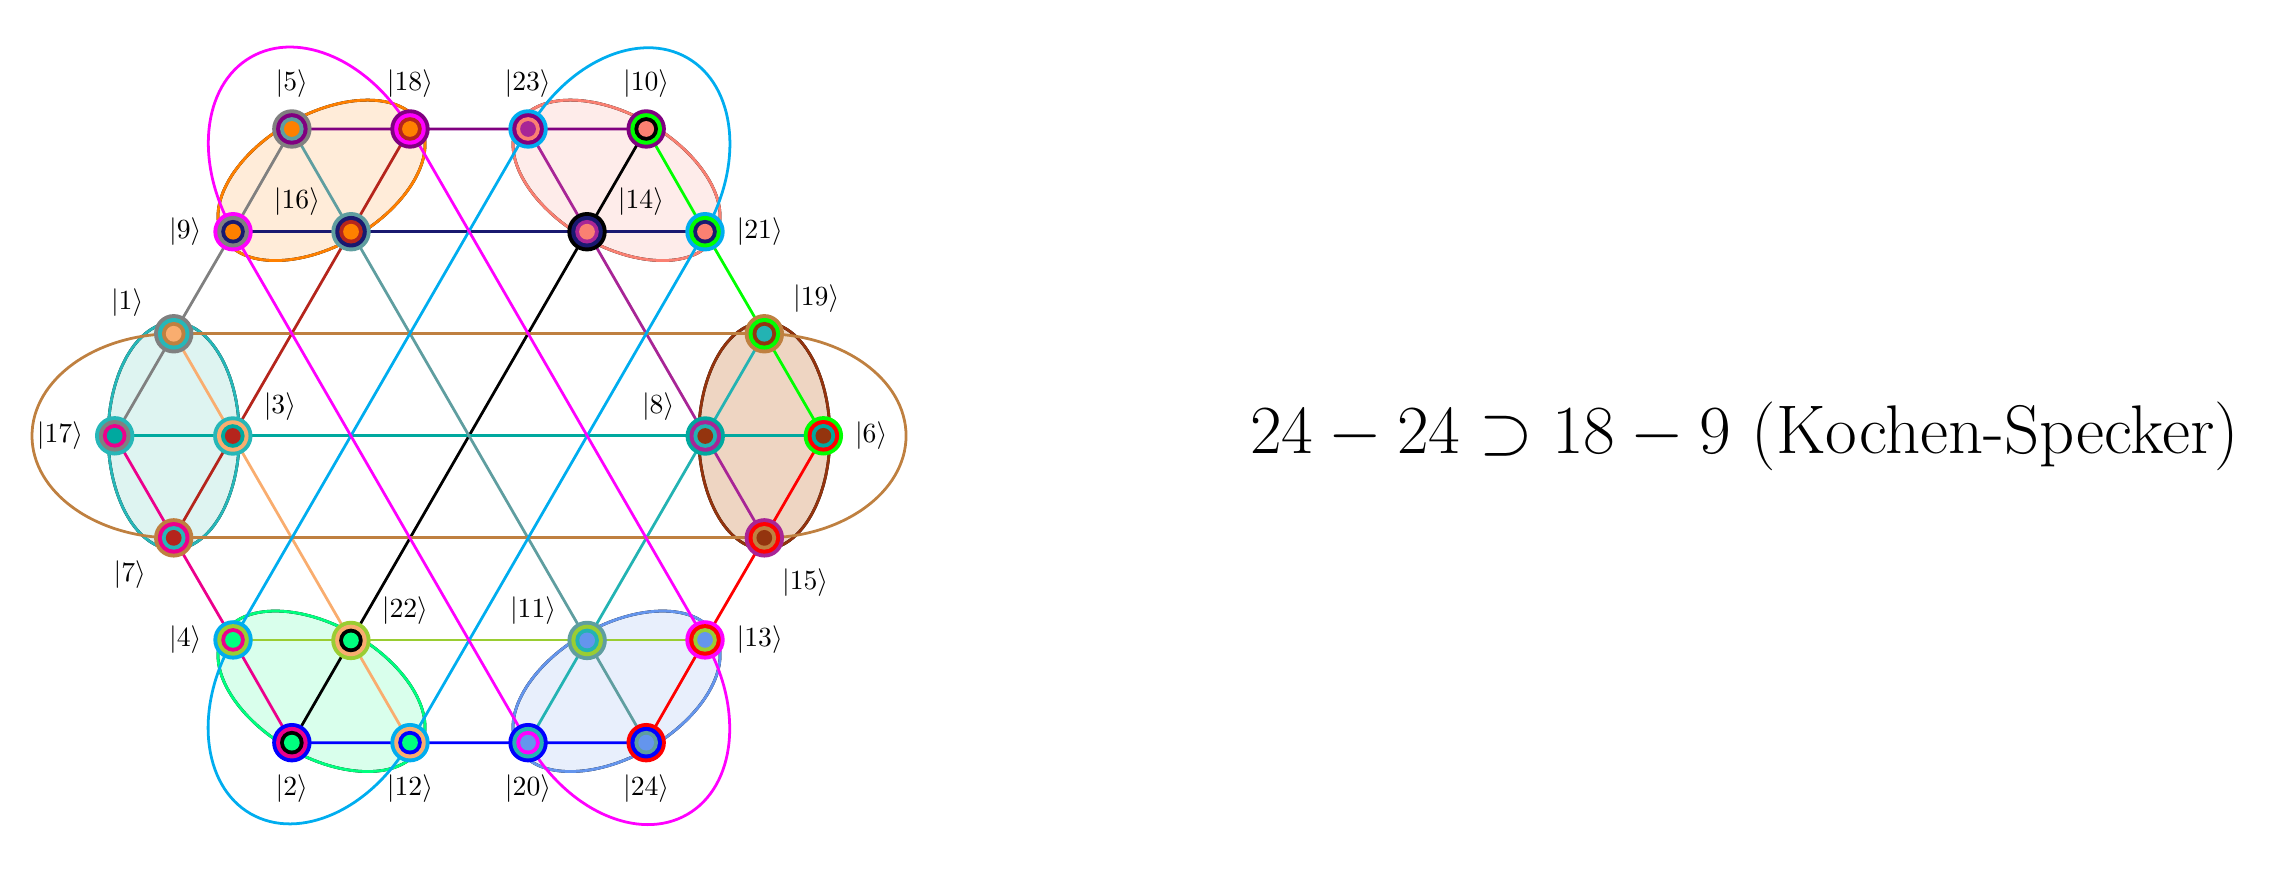
\begin{tikzpicture}  [scale=0.9]
\tikzstyle{every path}=[line width=1pt]   %,label distance=0.6pt
\newdimen\ms
\ms=0.1cm
        %\tikzstyle{c2}=[circle,inner sep=1pt,minimum size=5pt]
        %\tikzstyle{c1}=[circle,inner sep=0pt,minimum size=3pt]
\tikzstyle{c4}=[circle,inner sep={\ms/8},minimum size=5*\ms]
\tikzstyle{c3}=[circle,inner sep={\ms/8},minimum size=4*\ms]
\tikzstyle{c2}=[circle,inner sep={\ms/8},minimum size=3*\ms]
\tikzstyle{c1}=[circle,inner sep={\ms/8},minimum size=2*\ms]



        %%% Define positions of some observables
        \path
              (240:5) coordinate(1)
              (-0.833,-4.33) coordinate(2)
              (0.833,-4.33) coordinate(3)
              (300:5) coordinate(4)
              (3.33,-2.88) coordinate(5)
              (4.167,-1.44) coordinate(6)
              (0:5) coordinate(7)
              (4.167,1.44) coordinate(8)
              (3.33,2.88) coordinate(9)
              (60:5) coordinate(10)
              (0.833,4.33) coordinate(11)
              (-0.833,4.33) coordinate(12)
              (120:5) coordinate(13)
              (-3.33,2.88) coordinate(14)
              (-4.167,1.44) coordinate(15)
              (180:5) coordinate(16)
              (-4.167,-1.44) coordinate(17)
              (-3.33,-2.88) coordinate(18);




        %%% Draw all the context curves

       % small ellipses

\node[ellipse, draw, fill=BlueGreen!15!white, minimum width=1.666cm, minimum height=2.88cm] at (-4.167,0) {};
\node[ellipse, draw, color=BlueGreen, minimum width=1.666cm, minimum height=2.88cm] at (-4.167,0) {};
\node[ellipse, draw, fill=RawSienna!15!white, minimum width=1.666cm, minimum height=2.88cm] at (4.167,0) {};
\node[ellipse, draw, color=RawSienna, minimum width=1.666cm, minimum height=2.88cm] at (4.167,0) {};
\node[ellipse, draw, fill=SpringGreen!15!white, minimum width=1.666cm, minimum height=2.88cm, rotate=60] at (-2.0815,-3.605) {};
\node[ellipse, draw, color=SpringGreen, minimum width=1.666cm, minimum height=2.88cm, rotate=60] at (-2.0815,-3.605) {};
\node[ellipse, draw, fill=Salmon!15!white, minimum width=1.666cm, minimum height=2.88cm, rotate=60] at ( 2.0815, 3.605) {};
\node[ellipse, draw, color=Salmon, minimum width=1.666cm, minimum height=2.88cm, rotate=60] at ( 2.0815, 3.605) {};
\node[ellipse, draw, fill=orange!15!=, minimum width=1.666cm, minimum height=2.88cm, rotate=-60] at (-2.0815, 3.605) {};
\node[ellipse, draw, color=orange, minimum width=1.666cm, minimum height=2.88cm, rotate=-60] at (-2.0815, 3.605) {};
\node[ellipse, draw, fill=CornflowerBlue!15!white, minimum width=1.666cm, minimum height=2.88cm, rotate=-60] at ( 2.0815, -3.605) {};
\node[ellipse, draw, color=CornflowerBlue, minimum width=1.666cm, minimum height=2.88cm, rotate=-60] at ( 2.0815, -3.605) {};


        % outer hexagons

\draw [color=green] (7) -- (8) -- (9)-- (10);
\draw [color=violet] (10) -- (11) -- (12) -- (13);
\draw [color=gray] (13) -- (14) -- (15) -- (16);
\draw [color=magenta] (16) -- (17) -- (18) -- (1);
\draw [color=blue] (1) -- (2) -- (3) -- (4);
\draw [color=red] (4) -- (5) -- (6) -- (7);

        % inner hexagons

\draw [color=Apricot] (2) -- (15);
\draw [color=TealBlue] (3) -- (8);
\draw [color=YellowGreen] (5) -- (18);
\draw [color=MidnightBlue] (9) -- (14);
\draw [color=Mulberry] (11) -- (6);
\draw [color=BrickRed] (12) -- (17);

       % inner diagonals


\draw [color=black] (1) -- (10);
\draw [color=Emerald] (7) -- (16);
\draw [color=CadetBlue] (4) -- (13);





      % outer ovals

        \draw [color=brown] (8) -- (15);
        \draw [color=brown](17) -- (6);
        \draw [color=brown] (8) arc (450:270:2 and 1.44);
        \draw [color=brown] (15) arc (90:270:2 and 1.44);

        \draw [color=cyan] (9) -- (2);
        \draw [color=cyan] (11) -- (18);
        \draw [rotate=240,color=cyan] (9) arc (90:270:2 and 1.44);
        \draw[rotate=60,color=cyan] (18) arc (90:270:2 and 1.44);

        \draw [color=Fuchsia] (12) -- (5);
        \draw [color=Fuchsia] (14) -- (3);
        \draw[rotate=300,color=Fuchsia] (12) arc (90:270:2 and 1.44);
        \draw[rotate=120,color=Fuchsia] (3) arc (90:270:2 and 1.44);




        % Draw the observables themselves
        \draw (1) coordinate[c4,fill=blue,label=270:$\vert 2 \rangle$];
        \draw (1) coordinate[c3,fill=magenta];
        \draw (1) coordinate[c2,fill=black];
        \draw (1) coordinate[c1,fill=SpringGreen];

        \draw (2) coordinate[c4,fill=cyan,label=270:$\vert 12 \rangle$];
        \draw (2) coordinate[c3,fill=Apricot];
        \draw (2) coordinate[c2,fill=blue];
        \draw (2) coordinate[c1,fill=SpringGreen];

        \draw (3) coordinate[c4,fill=blue,label=270:$\vert 20 \rangle$];
        \draw (3) coordinate[c3,fill=TealBlue];
        \draw (3) coordinate[c2,fill=Fuchsia];
        \draw (3) coordinate[c1,fill=CornflowerBlue];

        \draw (4) coordinate[c4,fill=red,label=270:$\vert 24 \rangle$];
        \draw (4) coordinate[c3,fill=blue];
        \draw (4) coordinate[c2,fill=CadetBlue];
        \draw (4) coordinate[c1,fill=CornflowerBlue];

        \draw (5) coordinate[c4,fill=Fuchsia,label=0:$\vert 13 \rangle$];
        \draw (5) coordinate[c3,fill=red];
        \draw (5) coordinate[c2,fill=YellowGreen];
        \draw (5) coordinate[c1,fill=CornflowerBlue];

        \draw (6) coordinate[c4,fill=Mulberry,label=290:$\vert 15 \rangle$];
        \draw (6) coordinate[c3,fill=red];
        \draw (6) coordinate[c2,fill=brown];
        \draw (6) coordinate[c1,fill=RawSienna];

        \draw (7) coordinate[c4,fill=green,label=0:$\vert 6 \rangle$];
        \draw (7) coordinate[c3,fill=red];
        \draw (7) coordinate[c2,fill=Emerald];
        \draw (7) coordinate[c1,fill=RawSienna];

        \draw (8) coordinate[c4,fill=brown,label=30:$\vert 19 \rangle$];
        \draw (8) coordinate[c3,fill=green];
        \draw (8) coordinate[c2,fill=RawSienna];
        \draw (8) coordinate[c1,fill=TealBlue];

        \draw (9) coordinate[c4,fill=cyan,label=0:$\vert 21 \rangle$];
        \draw (9) coordinate[c3,fill=green];
        \draw (9) coordinate[c2,fill=MidnightBlue];
        \draw (9) coordinate[c1,fill=Salmon];

        \draw (10) coordinate[c4,fill=violet,label=90:$\vert 10 \rangle$];
        \draw (10) coordinate[c3,fill=green];
        \draw (10) coordinate[c2,fill=black];
        \draw (10) coordinate[c1,fill=Salmon];

        \draw (11) coordinate[c4,fill=cyan,label=91:$\vert 23 \rangle$];
        \draw (11) coordinate[c3,fill=violet];
        \draw (11) coordinate[c2,fill=Salmon];
        \draw (11) coordinate[c1,fill=Mulberry];

        \draw (12) coordinate[c4,fill=violet,label=90:$\vert 18 \rangle$];
        \draw (12) coordinate[c3,fill=Fuchsia];
        \draw (12) coordinate[c2,fill=BrickRed];
        \draw (12) coordinate[c1,fill=orange];

        \draw (13) coordinate[c4,fill=gray,label=90:$\vert 5 \rangle$];
        \draw (13) coordinate[c3,fill=violet];
        \draw (13) coordinate[c2,fill=CadetBlue];
        \draw (13) coordinate[c1,fill=orange];

        \draw (14) coordinate[c4,fill=Fuchsia,label=180:$\vert 9 \rangle$];
        \draw (14) coordinate[c3,fill=gray];
        \draw (14) coordinate[c2,fill=MidnightBlue];
        \draw (14) coordinate[c1,fill=orange];

        \draw (15) coordinate[c4,fill=gray,label=160:$\vert 1 \rangle$];
        \draw (15) coordinate[c3,fill=BlueGreen];
        \draw (15) coordinate[c2,fill=brown];
        \draw (15) coordinate[c1,fill=Apricot];

        \draw (16) coordinate[c4,fill=BlueGreen,label=180:$\vert 17 \rangle$];
        \draw (16) coordinate[c3,fill=gray];
        \draw (16) coordinate[c2,fill=magenta];
        \draw (16) coordinate[c1,fill=Emerald];

        \draw (17) coordinate[c4,fill=brown,label=215:$\vert 7 \rangle$];
        \draw (17) coordinate[c3,fill=magenta];
        \draw (17) coordinate[c2,fill=BlueGreen];
        \draw (17) coordinate[c1,fill=BrickRed];

        \draw (18) coordinate[c4,fill=cyan,label=180:$\vert 4 \rangle$];
        \draw (18) coordinate[c3,fill=YellowGreen];
        \draw (18) coordinate[c2,fill=magenta];
        \draw (18) coordinate[c1,fill=SpringGreen];


\node (19) at ($(2)!0.25!(15)$) {};  \draw (19) coordinate[c4,fill=YellowGreen,label=15:$\vert 22 \rangle$];
\node (20) at ($(3)!0.25!(8)$) {};   \draw (20) coordinate[c4,fill=CadetBlue,label=165:$\vert 11 \rangle$];
\node (21) at ($(3)!0.75!(8)$) {};   \draw (21) coordinate[c4,fill=Emerald,label=165:$\vert 8 \rangle$];
\node (22) at ($(9)!0.25!(14)$) {};  \draw (22) coordinate[c4,fill=black,label=15:$\vert 14 \rangle$];
\node (23) at ($(9)!0.75!(14)$) {};   \draw (23) coordinate[c4,fill=CadetBlue,label=165:$\vert 16 \rangle$];
\node (24) at ($(2)!0.75!(15)$) {};  \draw (24) coordinate[c4,fill=BlueGreen,label=15:$\vert 3 \rangle$];

        \draw (19) coordinate[c3,fill=Apricot];
        \draw (19) coordinate[c2,fill=black];
        \draw (19) coordinate[c1,fill=SpringGreen];

        \draw (20) coordinate[c3,fill=YellowGreen];
        \draw (20) coordinate[c2,fill=TealBlue];
        \draw (20) coordinate[c1,fill=CornflowerBlue];

        \draw (21) coordinate[c3,fill=Mulberry];
        \draw (21) coordinate[c2,fill=TealBlue];
        \draw (21) coordinate[c1,fill=RawSienna];

        \draw (22) coordinate[c3,fill=MidnightBlue];
        \draw (22) coordinate[c2,fill=Mulberry];
        \draw (22) coordinate[c1,fill=Salmon];

        \draw (23) coordinate[c3,fill=MidnightBlue];
        \draw (23) coordinate[c2,fill=BrickRed];
        \draw (23) coordinate[c1,fill=orange];

        \draw (24) coordinate[c3,fill=Apricot];
        \draw (24) coordinate[c2,fill=Emerald];
        \draw (24) coordinate[c1,fill=BrickRed];





        % Context labels
%\node[draw=none,color=blue] at (0,-6) {$a$};
%\node[draw=none,color=red] at (6,-3) {$b$};
%\node[draw=none,color=green] at (6,3) {$c$};
%\node[draw=none,color=violet] at (0,6) {$d$};
%\node[draw=none,color=gray] at (-6,3) {$e$};
%\node[draw=none,color=magenta] at (-6,-3) {$f$};
%\node[draw=none,color=cyan] at (-0.8,0.7) {$i$};
%\node[draw=none,color=Fuchsia] at (0.8,0.7) {$h$};
%\node[draw=none,color=brown] at (0,-0.9) {$g$};


\node[draw=none,color=black] at (18,0) {\Huge $24-24 \supset  18-9$ (Kochen-Specker)};
    \end{tikzpicture}
}
\end{center}
\end{frame}





\subsection{Case study II: Matrix pencil of the Greenberger-Horne-Zeilinger-Mermin argument}

\begin{frame}%[shrink=2]
 \frametitle{Case study II: Matrix pencil of the Greenberger-Horne-Zeilinger-Mermin argument}

\[
a
\sigma_x \myotimes  \sigma_x \myotimes  \sigma_x+
b
\sigma_y \myotimes  \sigma_y \myotimes  \sigma_x+
c
\sigma_y \myotimes  \sigma_x \myotimes  \sigma_y+
d
\sigma_x \myotimes  \sigma_y \myotimes  \sigma_y
\]

{\scriptsize

%\resizebox{.4\textwidth}{!}{
$$
\begin{aligned}
\pm (a - b - c - d):
\vert \text{GHZ}_{1,2} \rangle =& \frac{1}{\sqrt{2}}\left( \vert z_+z_+z_+ \rangle  \pm  \vert z_-z_-z_- \rangle \right)
   = \frac{1}{\sqrt{2}}\begin{pmatrix} 1, 0, 0, 0, 0, 0, 0, \pm 1 \end{pmatrix}^\intercal ,  \\
%-a + b + c + d:
%\vert \text{GHZ}_2 \rangle =& \frac{1}{\sqrt{2}}\left( \vert z_+z_+z_+ \rangle  - \vert z_-z_-z_- \rangle \right)
%   = \frac{1}{\sqrt{2}}\begin{pmatrix} 1, 0, 0, 0, 0, 0, 0, -1 \end{pmatrix}^\intercal , \\
\pm (a - b + c + d):
\vert \text{GHZ}_{3,4} \rangle =& \frac{1}{\sqrt{2}}\left( \vert z_+z_+z_- \rangle  \pm \vert z_-z_-z_+ \rangle \right)
   = \frac{1}{\sqrt{2}}\begin{pmatrix} 0, 1, 0, 0, 0, 0, \pm 1, 0 \end{pmatrix}^\intercal ,  \\
%-a + b - c - d:
%\vert \text{GHZ}_4 \rangle =& \frac{1}{\sqrt{2}}\left( \vert z_+z_+z_- \rangle  - \vert z_-z_-z_+ \rangle \right)
%   = \frac{1}{\sqrt{2}}\begin{pmatrix} 0, 1, 0, 0, 0, 0, -1, 0 \end{pmatrix}^\intercal , \\
\pm (a + b - c + d):
\vert \text{GHZ}_{5,6} \rangle =& \frac{1}{\sqrt{2}}\left( \vert z_+z_-z_+ \rangle  \pm  \vert z_-z_+z_- \rangle \right)
   = \frac{1}{\sqrt{2}}\begin{pmatrix} 0, 0, 1, 0, 0, \pm 1, 0, 0 \end{pmatrix}^\intercal ,  \\
%-a - b + c - d:
%\vert \text{GHZ}_6 \rangle =& \frac{1}{\sqrt{2}}\left( \vert z_+z_-z_+ \rangle  - \vert z_-z_+z_- \rangle \right)
%   = \frac{1}{\sqrt{2}}\begin{pmatrix} 0, 0, 1, 0, 0, -1, 0, 0 \end{pmatrix}^\intercal , \\
\pm ( a + b + c - d):
\vert \text{GHZ}_{7,8} \rangle =& \frac{1}{\sqrt{2}}\left( \vert z_+z_-z_- \rangle  \pm  \vert z_-z_+z_+ \rangle \right)
   = \frac{1}{\sqrt{2}}\begin{pmatrix} 0, 0, 0, 1, \pm 1, 0, 0, 0 \end{pmatrix}^\intercal ,  \\
%-a - b - c + d:
%\vert \text{GHZ}_8 \rangle =& \frac{1}{\sqrt{2}}\left( \vert z_+z_-z_- \rangle  - \vert z_-z_+z_+ \rangle \right)
%   = \frac{1}{\sqrt{2}}\begin{pmatrix} 0, 0, 0, 1,- 1, 0, 0, 0 \end{pmatrix}^\intercal .
\end{aligned}
$$
%}
}

\begin{center}
\resizebox{1\textwidth}{!}{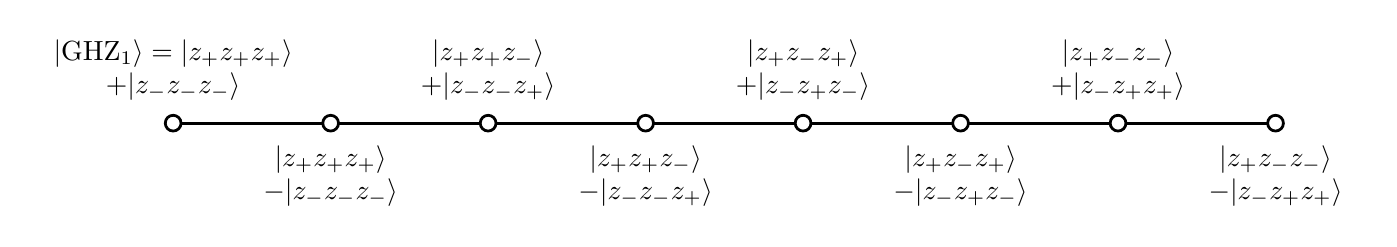
\begin{tikzpicture}  [scale=2]

\tikzstyle{every path}=[line width=1pt]

\newdimen\ms
\ms=0.1cm
\tikzstyle{s1}=[color=red,rectangle,inner sep=3.5]
\tikzstyle{c3}=[circle,inner sep={\ms/8},minimum size=4*\ms]
\tikzstyle{c2}=[circle,inner sep={\ms/8},minimum size=3*\ms]
\tikzstyle{c1}=[circle,inner sep={\ms/8},minimum size=2*\ms]
\tikzstyle{cs1}=[circle,inner sep={\ms/8},minimum size=1*\ms]

% Define positions of all observables

\coordinate (uuu) at (0,8);
\coordinate (uuv) at (1,8);
\coordinate (uvu) at (2,8);
\coordinate (uvv) at (3,8);
\coordinate (vuu) at (4,8);
\coordinate (vuv) at (5,8);
\coordinate (vvu) at (6,8);
\coordinate (vvv) at (7,8);

% draw contexts

\draw [color=black] (uuu) -- (vvv);

% draw atoms

\draw (uuu) coordinate[c1,fill=white, draw=black,label=above:{\begin{tabular}{c} $\vert \text{GHZ}_1 \rangle =\vert z_+z_+z_+ \rangle $\\$ + \vert z_-z_-z_- \rangle $\end{tabular}}];
\draw (uuv) coordinate[c1,fill=white, draw=black,label=below:{\begin{tabular}{c} $\vert z_+z_+z_+ \rangle $\\$ - \vert z_-z_-z_- \rangle $\end{tabular}}];
\draw (uvu) coordinate[c1,fill=white, draw=black,label=above:{\begin{tabular}{c} $\vert z_+z_+z_- \rangle $\\$ + \vert z_-z_-z_+ \rangle $\end{tabular}}];
\draw (uvv) coordinate[c1,fill=white, draw=black,label=below:{\begin{tabular}{c} $\vert z_+z_+z_- \rangle $\\$ - \vert z_-z_-z_+ \rangle $\end{tabular}}];
\draw (vuu) coordinate[c1,fill=white, draw=black,label=above:{\begin{tabular}{c} $\vert z_+z_-z_+ \rangle $\\$ + \vert z_-z_+z_- \rangle $\end{tabular}}];
\draw (vuv) coordinate[c1,fill=white, draw=black,label=below:{\begin{tabular}{c} $\vert z_+z_-z_+ \rangle $\\$ - \vert z_-z_+z_- \rangle $\end{tabular}}];
\draw (vvu) coordinate[c1,fill=white, draw=black,label=above:{\begin{tabular}{c} $\vert z_+z_-z_- \rangle $\\$ + \vert z_-z_+z_+ \rangle $\end{tabular}}];
\draw (vvv) coordinate[c1,fill=white, draw=black,label=below:{\begin{tabular}{c} $\vert z_+z_-z_- \rangle $\\$ - \vert z_-z_+z_+ \rangle $\end{tabular}}];


\end{tikzpicture}
}
\end{center}

\end{frame}


\subsection{Case study III: Matrix pencil of two-partite Greenberger-Horne-Zeilinger argument}

\begin{frame}%[shrink=2]
 \frametitle{Case study III: Matrix pencil of two-partite Greenberger-Horne-Zeilinger argument}

\[
a
(\sigma_z \myotimes \sigma_x) \cdot (\sigma_x \myotimes \sigma_z)
+b
\sigma_x\myotimes \sigma_x
+c
\sigma_z\myotimes \sigma_z
\]

{\scriptsize

%\resizebox{.4\textwidth}{!}{
$$
\begin{aligned}
-a - b - c:
\vert \Psi_- \rangle =& \frac{1}{\sqrt{2}}\left( \vert z_+z_- \rangle  -  \vert z_-z_+ \rangle \right)
   = \frac{1}{\sqrt{2}}\begin{pmatrix} 0,1, -1,0 \end{pmatrix}^\intercal ,  \\
a + b - c:
\vert \Psi_+ \rangle =& \frac{1}{\sqrt{2}}\left( \vert z_+z_- \rangle  +  \vert z_-z_+ \rangle \right)
   = \frac{1}{\sqrt{2}}\begin{pmatrix} 0,1, 1,0 \end{pmatrix}^\intercal ,  \\
a - b + c:
\vert \Phi_- \rangle =& \frac{1}{\sqrt{2}}\left( \vert z_+z_+ \rangle  -  \vert z_-z_- \rangle \right)
   = \frac{1}{\sqrt{2}}\begin{pmatrix} 1,0,0, -1 \end{pmatrix}^\intercal ,  \\
-a + b + c:
\vert \Phi_+ \rangle =& \frac{1}{\sqrt{2}}\left( \vert z_+z_+ \rangle  +  \vert z_-z_- \rangle \right)
   = \frac{1}{\sqrt{2}}\begin{pmatrix} 1,0,0, 1 \end{pmatrix}^\intercal ,  \\
\end{aligned}
$$
%}
}

\begin{center}
\resizebox{0.5\textwidth}{!}{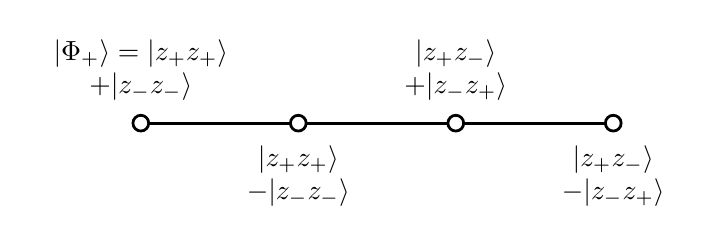
\begin{tikzpicture}  [scale=2]

\tikzstyle{every path}=[line width=1pt]

\newdimen\ms
\ms=0.1cm
\tikzstyle{s1}=[color=red,rectangle,inner sep=3.5]
\tikzstyle{c3}=[circle,inner sep={\ms/8},minimum size=4*\ms]
\tikzstyle{c2}=[circle,inner sep={\ms/8},minimum size=3*\ms]
\tikzstyle{c1}=[circle,inner sep={\ms/8},minimum size=2*\ms]
\tikzstyle{cs1}=[circle,inner sep={\ms/8},minimum size=1*\ms]

% Define positions of all observables

\coordinate (uuu) at (0,8);
\coordinate (uuv) at (1,8);
\coordinate (uvu) at (2,8);
\coordinate (uvv) at (3,8);
\coordinate (vuu) at (4,8);
\coordinate (vuv) at (5,8);
\coordinate (vvu) at (6,8);
\coordinate (vvv) at (7,8);

% draw contexts

\draw [color=black] (uuu) -- (uvv);

% draw atoms

\draw (uuu) coordinate[c1,fill=white, draw=black,label=above:{\begin{tabular}{c} $\vert \Phi_+ \rangle
=\vert z_+z_+ \rangle $\\$ + \vert z_-z_- \rangle $\end{tabular}}];
\draw (uuv) coordinate[c1,fill=white, draw=black,label=below:{\begin{tabular}{c} $\vert z_+z_+ \rangle $\\$ - \vert z_-z_- \rangle $\end{tabular}}];
\draw (uvu) coordinate[c1,fill=white, draw=black,label=above:{\begin{tabular}{c} $\vert z_+z_- \rangle $\\$ + \vert z_-z_+ \rangle $\end{tabular}}];
\draw (uvv) coordinate[c1,fill=white, draw=black,label=below:{\begin{tabular}{c} $\vert z_+z_- \rangle $\\$ - \vert z_-z_+ \rangle $\end{tabular}}];


\end{tikzpicture}
}
\end{center}

\end{frame}

\frame{

\centerline{\Large {\color{magenta} Thank you for your attention!}}

\begin{center}\color{orange}
$\widetilde{\qquad \qquad }$
$\widetilde{\qquad \qquad}$
$\widetilde{\qquad \qquad }$
\end{center}
 }
 \end{document}


















\section{ }

\frame{
 \frametitle{ }

\begin{itemize}
\item[$\bullet$] {
%\color{purple}
}
\pause
\item[$\bullet$] {
%\color{purple}
}
\end{itemize}
}

\section{ }

\frame{
 \frametitle{ }

\begin{itemize}
\item[$\bullet$] {
%\color{purple}
}
\pause
\item[$\bullet$] {
%\color{purple}
}
\end{itemize}
}

\section{ }

\frame{
 \frametitle{ }

\begin{itemize}
\item[$\bullet$] {
%\color{purple}
}
\pause
\item[$\bullet$] {
%\color{purple}
}
\end{itemize}
}

\section{ }

\frame{
 \frametitle{ }

\begin{itemize}
\item[$\bullet$] {
%\color{purple}
}
\pause
\item[$\bullet$] {
%\color{purple}
}
\end{itemize}
}

